\section{Studio della Lunghezza di Autocorrelazione}\label{Parte C}
\begin{wrapfigure}{r}{0.3\textwidth}
\vspace{-25pt} 
  \begin{center}
	\includegraphics[width=0.28\textwidth]{Immagini/Reticolo}
  \end{center}
       \vspace{-15pt} 
       \caption[Campionatura per la Funzione di Correlazione.]{\footnotesize Campionatura per la Funzione di Correlazione.}\label{fig: simmetrie}
       \vspace{-15pt} 
\end{wrapfigure}

Per correlazione si intende una relazione tra variabili casuali tale per cui a ciascun valore assunto dalla prima variabile corrisponde, con una certa probabilità, un valore della seconda.
Nel capitolo \ref{Parte B} è già stata introdotta una misura di correlazione, il tempo di autocorrelazione $\tau$, che misura la similitudine delle osservabili microscopiche tra due configurazioni campionate a tempo diverso.

In questo capitolo verrà studiata un'altra misura di correlazione, le variabili prese in considerazione saranno la coppia $S_0$, spin medio su una  generica riga del reticolo e $S_t$, spin medio su una seconda riga posta a $t$ passi reticolari dalla riga scelta. 
Lo scopo di questa analisi è di stimare fino a quale distanza lo spin in un punto riesce ad influenzare lo stato di un'altro nodo del sistema, questo tipo di interazione è totalmente indiretta visto che l'Hamiltoniana prevede solo interazioni tra siti primi vicini.

Per quantificare la correlazione tra righe diverse è necessario introdurre una funzione di correlazione, definita in modo simile alla funzione precedente:

\begin{equation}\label{eq: G_c}
G_c(t) = \dfrac{\langle S_i S_{i+t}\rangle - \langle S_i\rangle \langle S_{i+t}\rangle  }{\langle S_i^2\rangle - \langle S_i\rangle \langle S_{i}\rangle} \simeq \dfrac{\langle S_i S_{i+t}\rangle}{\langle S_i^2\rangle}
\end{equation}
dove le medie vanno intese come medie su tutti i valori campionati dello spin medio su una riga.

Per via delle simmetrie rotazionali ( di $90^\circ$) e traslazionali ( di passi reticolari) del reticolo quadrato, per ogni configurazione simulata si avranno $2L$ coppie di misure su cui valutare la correlazione.
L'ultima uguglianza nell'equazione \ref{eq: G_c} è un'approssimazione valida per le temperature $T>Tc$ dove, teoricamente, la magnetizzazione è nulla. 

In questo caso la funzione di correlazione quantifica la probabilità che due righe poste a $t$ passi di distanza abbiano lo stesso valore di magnetizzazione, infatti quando le coppie di righe hanno lo stesso spin $G_c = 1$ invece quando le magnetizzazioni tendono ad essere discordi e concordi con la medesima probabilità si avrà $G_c \rightarrow 0 $.
\medskip

Esattamente come nel caso dell'autocorrelazione si attende che la funzione di correlazione tra righe decada esponenzialmente:
\begin{equation}
G_c(t) \simeq e^{-t/\xi}
\end{equation}
dove il coefficiente $\xi$ del decadimento viene chiamato \emph{lunghezza di correlazione}.
Ovviamente anche in questo caso $\xi$ equivale al valore di $t$ per cui la correlazione corrisponde ad $e^-1$, quindi la quantità $2 \xi$ è la distanza dopo cui due linee possono essere considerate scorrelate.
\begin{figure}[h!]
   \caption[ParteC$\_$StS0vst$\_$Cluster.cpp ]{Andamento del coefficiente di correlazione medio tra coppie di linee in funzione della distanza $t$ per vari valori di $\beta$.}\label{fig: Cluster_S0Stvst}
     \centering
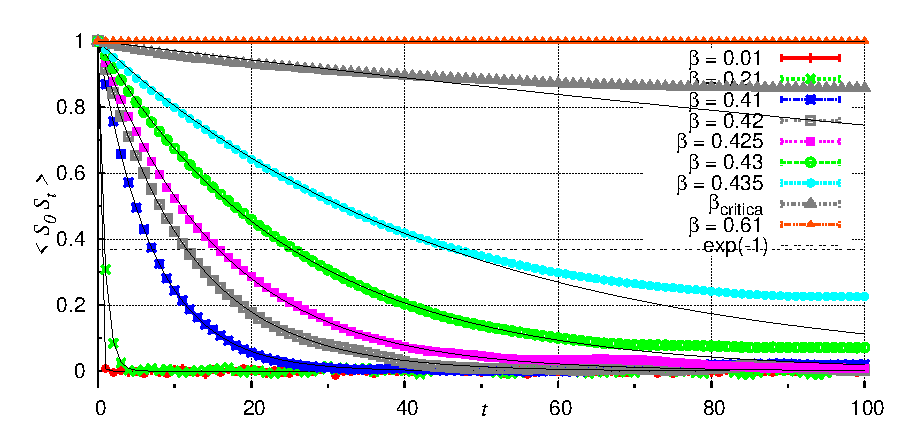
\includegraphics[width=1\textwidth]{Immagini/ParteC/Cluster_S0Stvst}
\end{figure}


\bigskip
Nella figura (\ref{fig: Cluster_S0Stvst}) è mostrato l'andamento della funzione di correlazione per uno stesso sistema simulato a $\beta$ crescenti fino al raggiungimento della temperatura critica (in questo intervallo è possibile usare l'espressione approssimata di $G_c$) dopo la fase critica il sistema è completamente magnetizzato, la maggior parte degli spin sono paralleli, e quindi il sistema risultarà sempre completamente correlato.
A ciascun set di dati è sovrapposto il fit esponenziale eseguito unicamente sui primi punti in modo da poter ignorare il comportamento rumoroso presente per alti valori di $t$.

Si noti come l'accordo con l'andamento esponenziale diminuisca al tendere di $\beta$ a $\beta_c$, l'effetto è dovuto al fatto che i modelli ad $L$ finito presentano una magnetizzazione residua anche alla temperatura critica laddove la soluzione teorica di Onsanger prevederebbe una magnetizzazione esattamente nulla(per tutte le temperature maggiori del valore critico).
\newline
Dal grafico è evidente come la lunghezza di correlazione, parametro $\xi$ che regola la concavità della funzione, cresca man mano che la temperatura diminuisce, dai fit esponenziali si ottengono le seguenti stime della lunghezza di correlazione:

\begin{center}
\begin{tabular}{|c|c |r c l| }
\hline
$\beta$	& $\xi$ \footnotesize{"ad occhio"}	&\multicolumn{3}{|c|}{$\xi_{fit}$	} \\
0,01	& $\sim$ 0,5	&0,20	&$\pm$	&0,01\\
0,21	& $\sim$ 1	&0,84	&$\pm$	&0,01\\
0,41	& $\sim$ 7	&7,11	&$\pm$	&0,02\\
0,42	& $\sim$ 11,5	&11,65	&$\pm$	&0,02\\
0,425	& $\sim$ 16	&15,75	&$\pm$	&0,04\\
0,43	& $\sim$ 25,5	&25,37	&$\pm$	&0,04\\
0,435	& $\sim$ 43,5	&45,79	&$\pm$	&0,11\\
critico	& oltre 100	&340,20	&$\pm$	&7,3\\
\hline
0,61	& $\infty$ 	& 	& $\infty$	& \\
\hline
\end{tabular}
\end{center}

Eseguendo questo stesso procedimento su una raccolta di dati più vasta( 80 valori di $\beta < \beta_c$) si può ottenere un grafico di $\xi$ in funzione di $X=\small \dfrac{\beta -\beta_c}{\beta_c}$( figura \ref{fig: XivsBeta}).

\begin{figure}[h!]
       \caption[ParteC$\_$StS0vst$\_$Moltitudini $\;\rightarrow\;$ molti\_S0Stvst.p ]{Andmaneto della lunghezza di correlazione in funzione della temperatura del sistema.}\label{fig: Xivst}
     \centering
		\includegraphics[width=0.70\textwidth]{Immagini/ParteC/xivst}

\footnotesize  $L= 200$ , $N_{configurazioni} = 100$
\end{figure}

Dal grafico è evidente come il valore della lunghezza di correlazione diverga molto velocemente avvicinandosi alla temperatura critica.
L'andamento ha tendenzialmente un buon accordo con $1/X$ fino al valore critico dove, in conseguenza alla dimensione finita del reticolo, la divergenza è limitata ad un valore massimo $\xi_L(\beta_c)$ grande ma finito.

\subsubsection*{Dipendenza di $\xi_L(\beta_c)$ da L}
Resta da determinare come il valore massimo $\xi_L(\beta_c)$ dipenda dalla dimensione del reticolo.
Per farlo si simulano vari sistemi con differente taglia del reticolo e si studia l'andamento della funzione di correlazione $G_c$ (approssimata) alla temperatura critica ( figura: \ref{fig: Cluster_Tc_S0Stvst} ).
Purtroppo l'accordo dell'espressione approssimata della funzione di correlazione con l'andamento esponenziale è molto debole a questa temperatura, si può comunque eseguire un fit esponenziale sui primi valori dei dati campionati ottenendo i seguenti valori:


     \begin{minipage}{0.3\textwidth}
		\begin{tabular}{|c|r c l| }
			\hline \footnotesize
			$\beta$	&\multicolumn{3}{|c|}{$\xi_{fit}$	} \\
330	&515,6	&$\pm$	&11,6\\
320	&384,7	&$\pm$	&6\\
310	&385,7	&$\pm$	&7,3\\
300	&278,69	&$\pm$	&4,5\\
290	&346,53	&$\pm$	& 7,5\\
280	&324,267	&$\pm$	& 6,6\\
270	&409,24	&$\pm$	& 10,51\\
260	&317,69	&$\pm$	& 6,8\\
250	&323,06	&$\pm$	& 6,5\\
240	&311,43	&$\pm$	& 7,1\\

\hline
\end{tabular}
     \end{minipage}\hfill
     \begin{minipage}{0.3\textwidth}
\begin{tabular}{|c|r c l| }
\hline \footnotesize
$\beta$	&\multicolumn{3}{|c|}{$\xi_{fit}$	} \\
230	&260,34	&$\pm$	& 4,864\\
220	&215,09	&$\pm$	& 3,23\\
210	&245,38	&$\pm$	& 4,69\\
200	&211,84	&$\pm$	& 3,43\\
190	&258,95	&$\pm$	& 5,76\\
180	&242,76	&$\pm$	& 6,12\\
170	&157	&$\pm$	& 1,98\\
160	&234,79	&$\pm$	& 5,31\\
150	&216,71	&$\pm$	& 5,36\\
140	&191,01	&$\pm$	& 4,21\\

\hline
\end{tabular}
     \end{minipage}\hfill
     \begin{minipage}{0.3\textwidth}
\begin{tabular}{|c|r c l| }
\hline \footnotesize
$\beta$	&\multicolumn{3}{|c|}{$\xi_{fit}$	} \\
130	&198,53	&$\pm$	& 4,95\\
120	&160,1	&$\pm$	& 3,55\\
110	&234	&$\pm$	& 8,88\\
100	&175,4	&$\pm$	& 4,63\\
90	&133,66	&$\pm$	& 3,79\\
80	&114,16	&$\pm$	& 2,81\\
70	&90,6	&$\pm$	& 2,43\\
60	&164,1	&$\pm$	& 8,22\\
50	&148,1	&$\pm$	& 7,44\\
40	&106,53	&$\pm$	& 5,66\\
\hline
\end{tabular}
     \end{minipage}\hfill

\begin{figure}[htbp]
      \centering
      \caption[ParteC\_Tc\_StS0vst\_Cluster.cpp ]{Andamento della funzione di Correlazione in funzione della distanza $t$ alla temperatura critica.}\label{fig: Cluster_Tc_S0Stvst}
	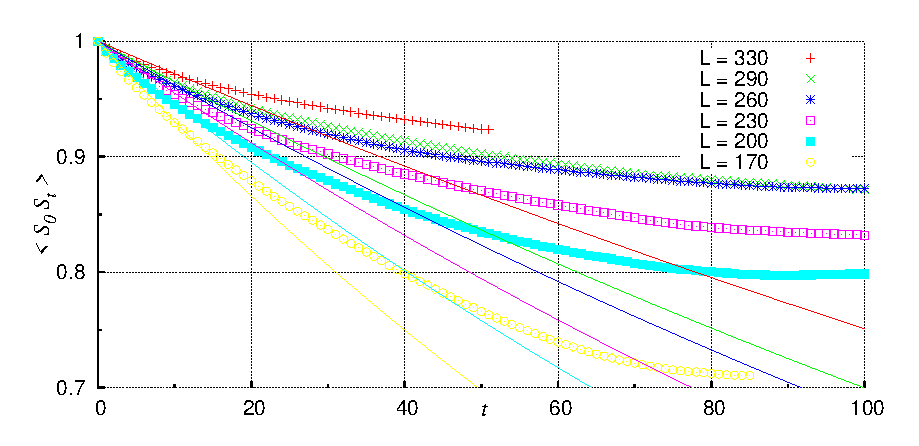
\includegraphics[width=1\textwidth]{Immagini/ParteC/Cluster_Tc_S0Stvst}
	\bigskip
	  \caption[ParteC\_Tc\_StS0vst\_Cluster.cpp $\;\rightarrow\;$ grafico\_file.p ]{Andamento della lunghezza di correlazione calcolata tramite il fit esponenziale dei grafici precedenti in funzione della taglia $L$.}\label{fig: grafpo_Tc}
	\includegraphics[width=1\textwidth]{Immagini/ParteC/grafpo_Tc}
\end{figure}
La dipendenza dei dati campionati di $\xi_L(\beta_c)$ da $L$ (figura \ref{fig: grafpo_Tc}) non è particolarmente regolare, ma si può notare (figure \ref{fig: Cluster_Tc_S0Stvst} e \ref{fig: grafpo_Tc}) come l'andamento sia distribuito in modo approsimativamente uniforme intorno ad una retta.
Si può concludere quindi che :
$$\xi_L(\beta_c) \simeq L $$
